\section{Methodology}

We intend to utilize the following methods:
\begin{itemize}
    \item[--] Exploratory analysis
    \item[--] Regression
    \item[--] ARIMA
    \item[--] LSTM --- Tensorflow
    \end{itemize}

\subsection{Data gathering}
In order to analyze the salmon price, we first need to gather this data on the salmon price.The main data point is the price of salmon. There are several sources for this data, but we utilized the data from the NASDAQ salmon exchange. The reason for this being a combination of the accessibility of the data, and the fact that the NASDAQ salmon exchange (NQSALMON) uses a weighted average for the salmon price, gathered from a spectrum of salmon exporters and it is therefore the best source of meaningful data. Another reason for using the NASDAQ salmon exchange is that the data is updated weekly with no missing values for the entire time frame. We downloaded data from March 2013 through December 2022, for a total of 507 data points. This was our base for the independent factors.The next step was to gather data from the other relevant factors for our analysis. 

\subsubsection{Norwegian fishermen and the market for wild caught fish}\label{Norwegian fishermen and the market for wild caught fish}
To understand where our price data comes from we need to take a look at how wild caught fish are sold in Norway. Wild caught fish in Norway have a heavily monitored way to the consumer. There are laws concerning quality and handling that secures the fish are safe to eat. There are also laws that dictate the way these fish can be sold and who are liable throughout this process. The laws concerning the sales are governed by the act on first hand purchace of wild marine resource. A sales organisation act like a middleman in the transaction between fisherman and fish buyer. They can be compared in likeness to an auction house or exchange, where the fisherman pays a fee to access the exchange to sell their fish. But the fishermen remain as owner of the fish until the time of the transaction. This means that the sales organistaion never actually own any of the fish. Through this sales process the Norwegian receipt for fishermen is created.\parencite{Nielsen_2022}

\subsubsection{Exchangeable goods}\label{Exchangeable goods}
We wanted to explore the possibility that one might be able to use prices for similar commodities such as different seafood to help predict the price of salmon. To find the prices of these exchangeable goods we contacted Norsk Råfisklag. They where very helpful and provided us with historic prices data for halibut and cod. The data they provided was gathered using the Norwegian receipt for fishermen also known as a contract note. The receipt is a concept that is unique to Norway. The receipt contains both the quantity of fish caught as well as the sales value of these fish and a plethora of other information. It has a number of porpoises like paying the fishermen, creating the invoice for the buyer, controlling that the quota of fish is upheld, contributing to the Norwegian statistics for wild caught fish, and more. We use data from these receipts to gather the week by week historic prices for halibut and cod. Norges Råfisklag witch provides the data is an entity created by the industry to make sure it upholds its responsibility to the rest of the society. It is also responsible for securing a fair and transparent industry for workers and the envoirement. This makes it a great reliable source of data.\parencite{Harland_2022}

\subsubsection{Currency change}\label{Currency change}
As mentioned the salmon market is an export market. This in turn means that the prices are affected by the changes in between the NOK and the currency of the markets that it is exported to. To account for this we have added Norges Bank's TWI to the dataset. ``The TWI is a nominal effective krone exchange rate calculated on the basis of NOK exchange rates against the currencies of Norway's 25 main trading partners.'' \parencite{norges_bank_2020} A rise in the value of the index indicates that the exchange rate of NOK depreciates.

\subsection{Exploratory analysis}

\subsection{Regression}

\subsection{Data preprocessing}
In order to use the data for prediction in our models we need to prepare the data. In our case this means to split the data into a training and test set. We will use the same split for all of our models, so that we they are comparable. The test set will be the last year of the data, 2021. The training set will be the rest of the data, 2013--2020. A very important aspect of forecasting using machine learning algorithms is that the test set should be `invisible' throughout the training process, otherwise we might get data leakage and consequently, a false sense of how well the model performs.~\parencite{brownlee_2016}
\subsection{ARIMA and SARIMAX}

As explained in~\ref{SeasonalityTheory} on page~\pageref{SeasonalityTheory}, one of the prerequisites for the ARIMA model is that the data is stationary. This can be done either by analysing the time-series itself and noticing the variance and trend, or by using the Augmented Dickey-Fuller test. 
After this is done, the next step will be to find the optimal parameters for the ARIMA model. This is usually done by looking at the ACF and PACF plots. 
When the optimal parameters are found, the model can be fitted and used to predict future values. \parencite{hyndman_athanasopoulos_2021}

\subsubsection{Determening stationarity}\label{DeterminingStationarity}
The Augmented Dickey-Fuller test is a statistical test that can be used to determine stationarity. The null hypothesis of the test is that the time-series is non-stationary. If the p-value is less than the significance level, the null hypothesis is rejected and the time-series is expected to be stationary.
Using the Augmented Dickey-Fuller test on the Salmon Price data, we get a p-value of 0.02406, this means that we can reject the null hypothesis at a 95\% confidence level according to this test. The data may therefore be stationary.~\parencite{Dickey_Fuller1979}

In order to better understand why the data is not stationary, we can plot the data and look at the variance, trend and seasonality. This is done by decomposing the data into its components. We then get the following plot: 

\begin{figure}[H]
    \centering
    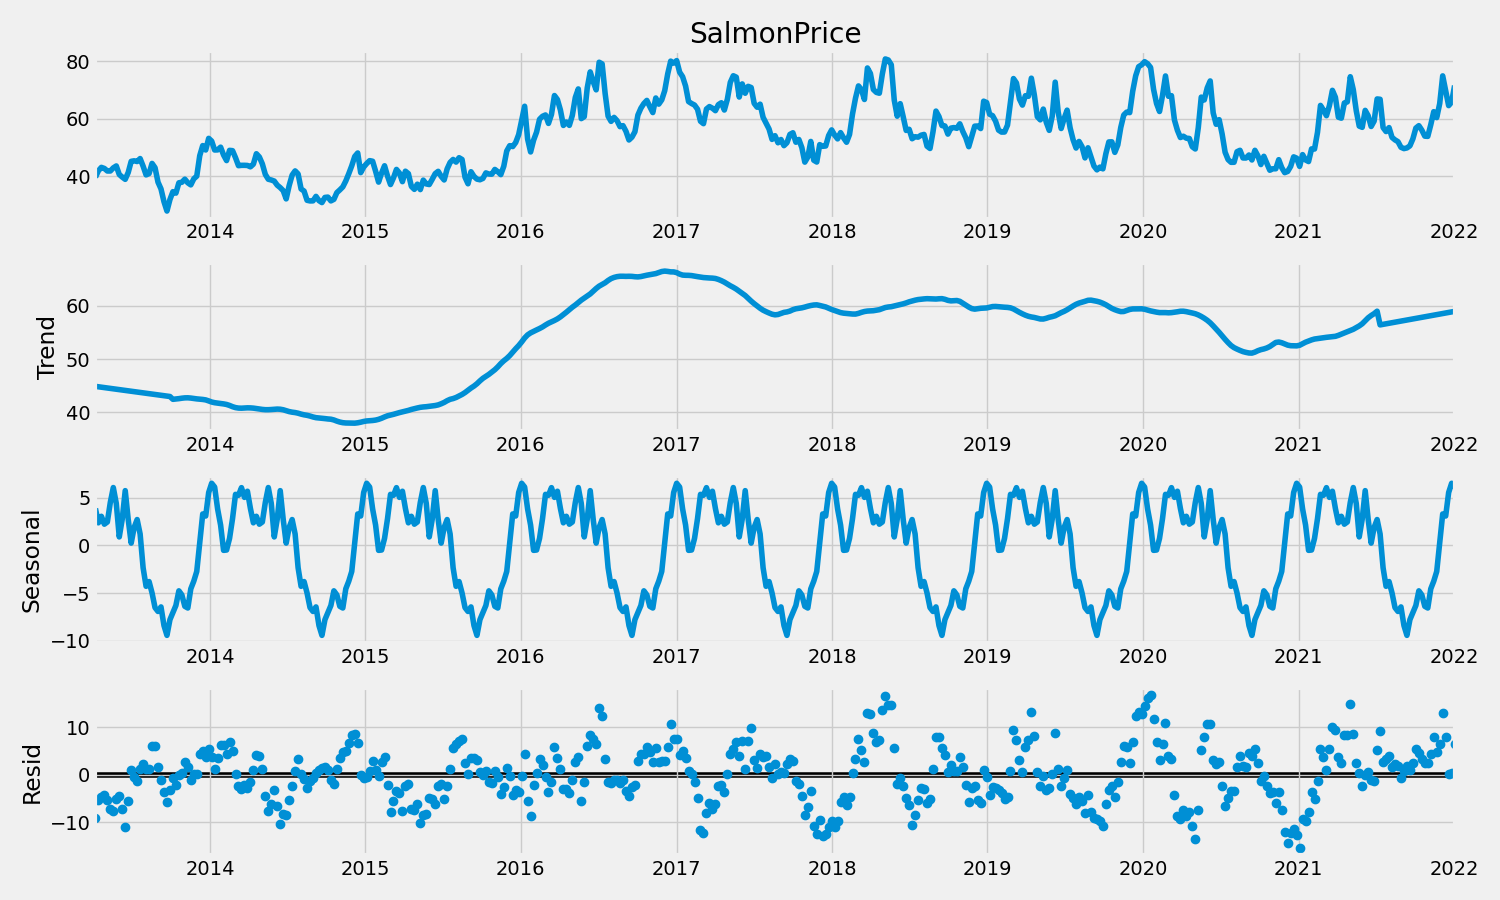
\includegraphics[width=0.8\textwidth]{data/Figures/ARIMA/Decomposition.png}
    \caption[Decomposition of the Salmon Price data]{Decomposition of the Salmon Price data.}\label{fig:Decomposition}
\end{figure}
Examining the decomposed data in Figure~\ref{fig:Decomposition} there are especially two things that stand out. The first is the trend, which is clearly increasing. The second is the seasonality, there is a clear yearly seasonal trend where the price is higher in the summer months before decreasing during the autumn and reaching a low in the winter. From this we draw a different conclusion than the Augmented Dickey-Fuller test, according to the plot, the data is not stationary and needs differencing. In the ARIMA model, this will be done by setting $d$ to 1 or more. 

The exact number of differencing needed can be found either by using the ADF-test on the differenced data and looking for when the p-value is less than the critical value, or by looking at the autocorrelation plot and using rules set out by \textcite{nau_2019} to determine the number of differencing needed. 
\begin{figure}[H]
    \centering
    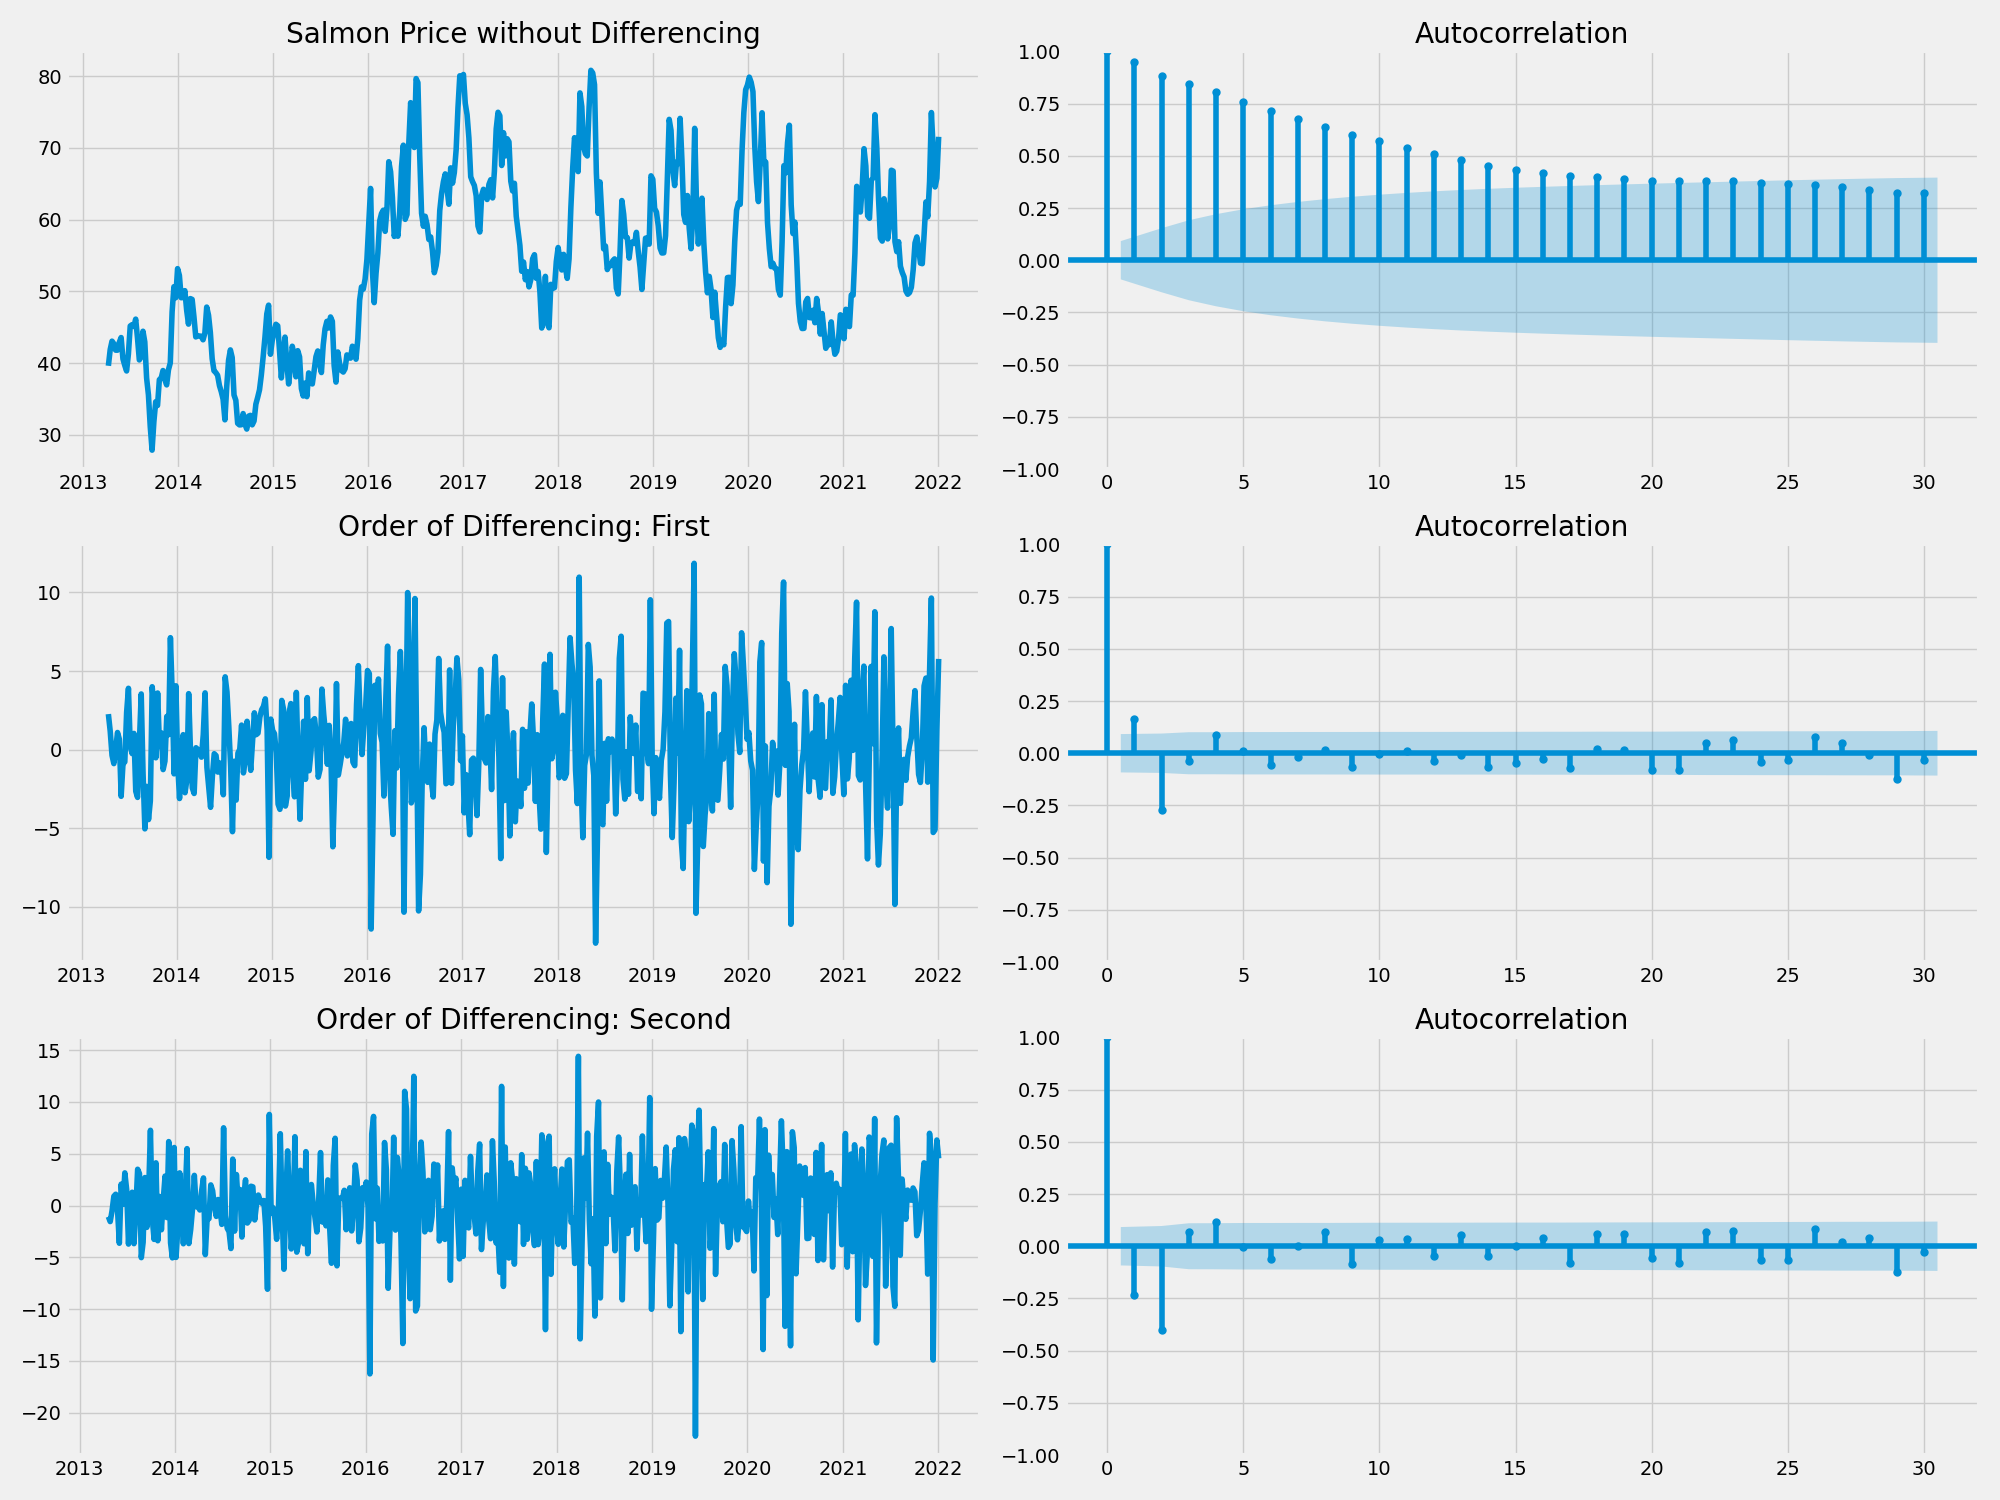
\includegraphics[width=0.8\textwidth]{data/Figures/ARIMA/Diff1_ACF_30.png}
    \caption[Different orders of differencing]{Different orders of differencing.}\label{fig:ACF_Differencing}
\end{figure}
Examining the trend and autocorrelation in Figure~\ref{fig:ACF_Differencing} we can see that the original data without differencing has both a clear trend and a slow decay in the autocorrelation plot with a high number of positive lags. Following the first rule from \textcite{nau_2019} we can conclude that the data needs at least one order of differencing.

After just a single order of differencing, the trends starts to flatten out and fluctuate around 0. The autocorrelation plot also drops sharply after the first lag, and is then quite small and patternless, this follows the second rule from \textcite{nau_2019} and will often be a sign that higher differencing is not needed. Running the Augmented Dickey-Fuller test on the differenced data, we get a p-value of 3.86388e-24, much lower than the critical value of 0.05. We can therefore reject the null hypothesis and conclude that the differenced data is stationary. 

With a second order of differencing, the trend seems to flatten even more, and the autocorrelation plot shows a sharp negative decline for the first and second lag, this may be a sign that the data is over-differenced. This is not optimal as over-differencing will lead to a loss of historical information and trends. It is therefore of utmost importance to find the order of differencing that both makes the data stationary and keeps the historical memory intact. Over-differencing is a common mistake when fitting non-stationary data to machine learning models, and can lead to the model not being able to capture the underlying trend.~\parencite{lopezde_prado2018}

A third way to determine the optimal number of differencing is, according to \textcite{nau_2019}, to look at the standard deviation of the plot at different orders of differencing. Following his rule number 3, the optimal number of differencing is the one where the standard deviation of the plot is the lowest. Examining Table~\ref{StdDevTable} we can see that the standard deviation of the data is lowest at the first order of differencing. After this the standard deviation increases, and there is no reason to believe any higher number of differencing will reduce the standard deviation. 

\begin{table}[H]
    \begin{center}
        \import{data/Figures/ARIMA/}{StdDevTable}
        \caption{\label{StdDevTable}Standard deviation of the differenced data.}
    \end{center}
\end{table}

We can therefore conclude that the optimal number of differencing should be either 0 or 1.

\subsubsection{Autoregression and Moving Average}
The next step in a regular ARIMA model is to identify the optimal AR and MA terms needed to fit the model. This can be done by comparing different models by looking at the AIC and BIC values, but with larger models this would constitute an unnecessary use of computational power. A more efficient way to find the optimal terms is to look at the ACF and PACF plots of the data and use the rules set out by \textcite{nau_2019} to determine the optimal $p$ and $q$. 
\begin{figure}[H]
    \centering
    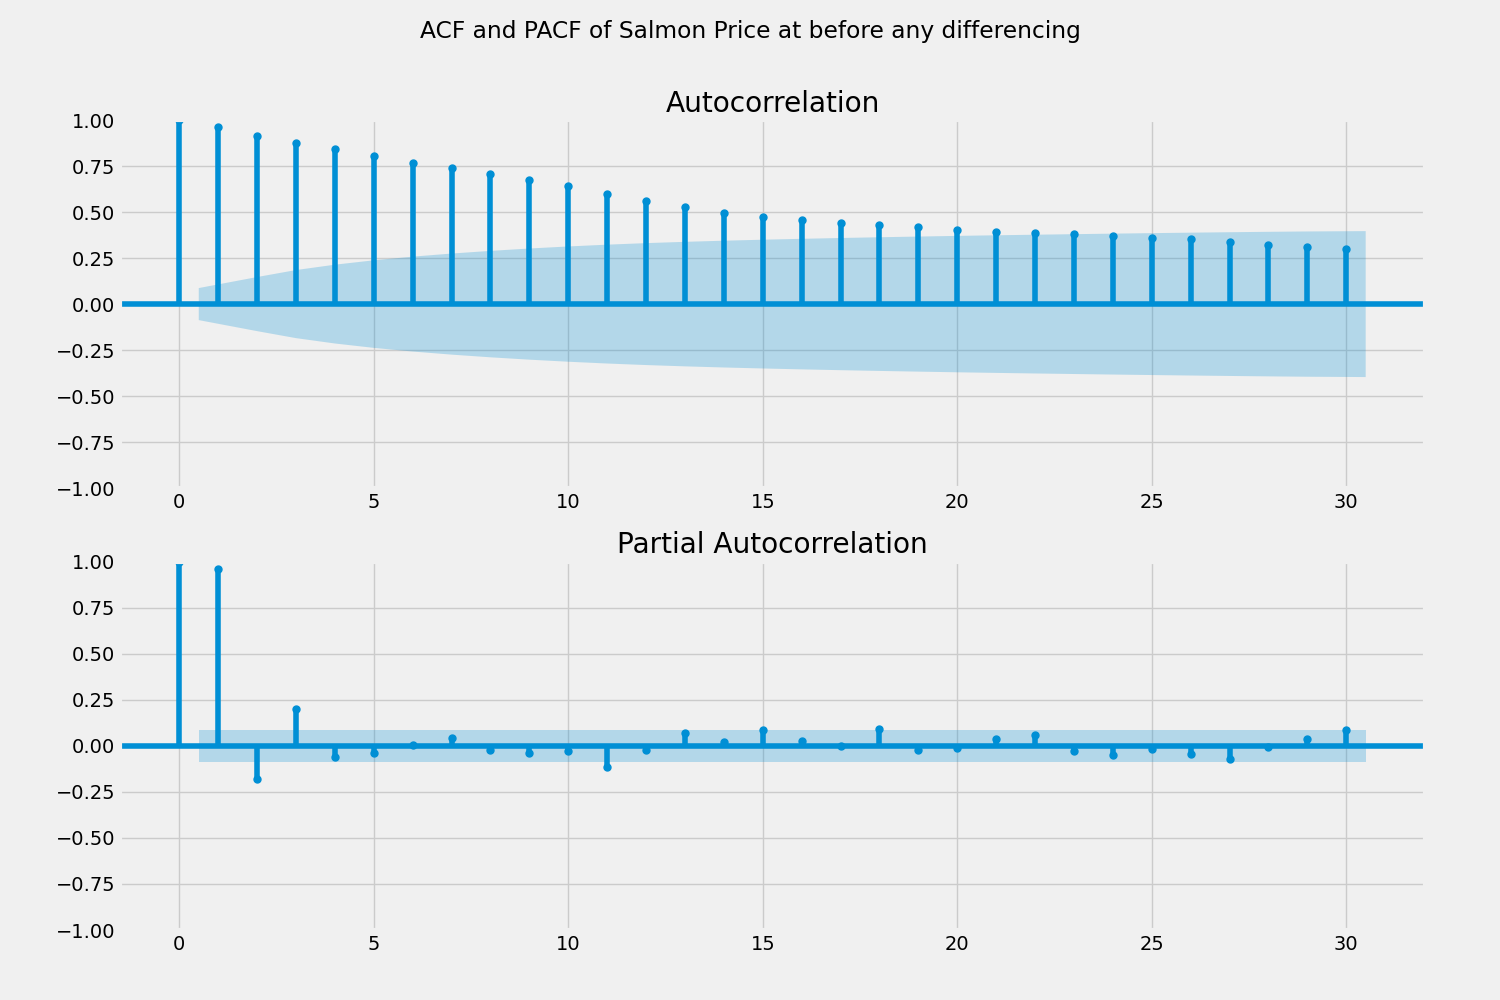
\includegraphics[width=0.8\textwidth]{data/Figures/ARIMA/OrigACF-PACF_30.png}
    \caption[ACF and PACF plots of Salmon price]{ACF and PACF plots of Salmon price.}\label{fig:Orig_ACF_PACF}
\end{figure}

The most noticeable part of the ACF plot in Figure~\ref{fig:Orig_ACF_PACF} is the slow decline of the autocorrelation after the first lag. This is a sign that the data is not white noise, and that there is a correlation between the data and its lags. According to \textcite{nau_2019}, this is called an `AR signature' and is a clear sign that we need to add an AR term to the model, rather than adding an MA term. To find the optimal amount of AR terms needed we can look at the PACF plot. As a rule of thumb, the optimal number is where the PACF plot exhibits a clear drop. In Figure~\ref{fig:Orig_ACF_PACF} we can see that the PACF plot drops sharply after the lag 1, and then fluctuates around 0, mostly within the confidence interval. Therefore, without any differencing, the optimal number of AR terms is 1. But, as we concluded in~\ref{DeterminingStationarity}, the data needs at least one order of differencing. We therefore need to look at the ACF and PACF plots of the differenced data.
\begin{figure}[H]
    \centering
    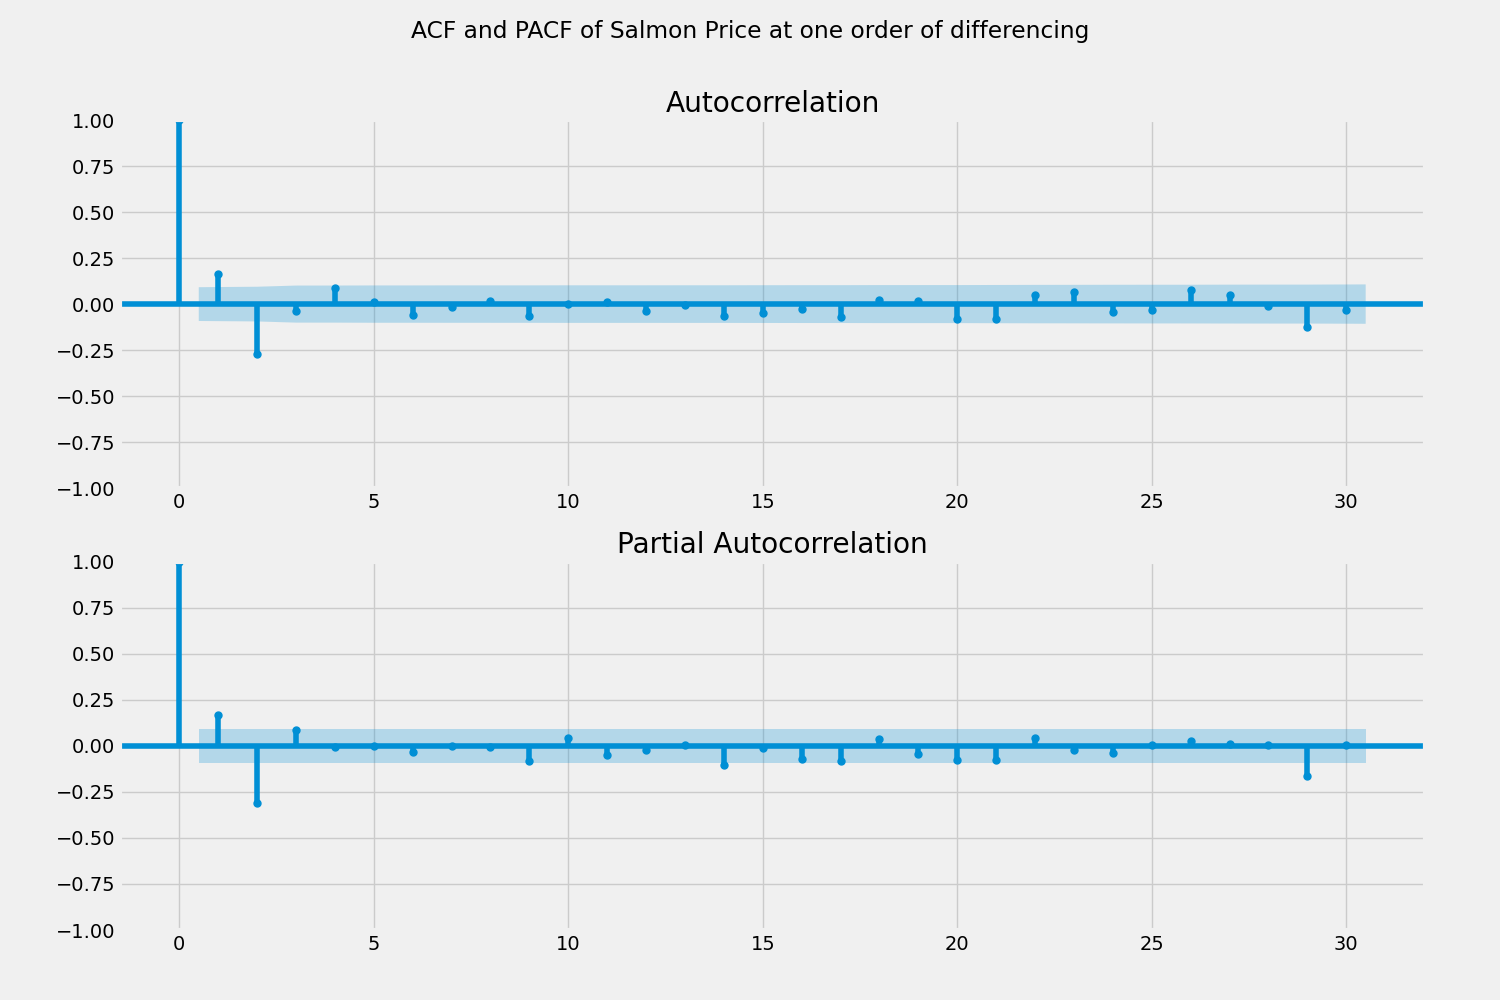
\includegraphics[width=0.8\textwidth]{data/Figures/ARIMA/DiffACF-PACF_30.png}
    \caption[ACF and PACF plots of differenced Salmon price]{ACF and PACF plots of differenced Salmon price.}\label{fig:Diff1_ACF_PACF}
\end{figure}

Examining the ACF plot in Figure~\ref{fig:Diff1_ACF_PACF} we can see that the autocorrelation now has a much more rapid decline compared to the original data. The PACF plot exhibits some of the same characteristics as the original data, but with a much sharper decline for the first lag. Nevertheless, as the first lag of both the ACF and PACF plot is positive and significant outside the 95\% confidence interval, there should be at least one AR term. At the same time, there is also some negative lags in both the ACF and PACF plots which may indicate that there should be an MA term, but according to \textcite{nau_2019}, we should be careful mixing AR and MA terms in ARIMA models, as they may cancel each other out. The best model will, in most cases, consist solely of either AR or MA terms.

As the interpretation of visual plots and clues from these can be a bit subjective, we should employ some objective test to determine the optimal number of $p$ and $q$. The most straight forward way to do this is to perform an iterative search over the possible values of $p$ and $q$ and then compare the AIC and BIC values of the different models, as well as comparing the mean squared error of the predictions from the models.  

\subsubsection{Seasonality}
Hitherto we have only considered the non-seasonal ARIMA model, but as with many time series, the Salmon price might also exhibit some seasonal patterns and trends. It may therefore be better to add a seasonal part to the model and consequently call it a SARIMA model. One way to determine this is to look at the seasonal part of the decomposed data. The decomposed data shows us what part of the variation in the data is due to the trend, the seasonal part, and the residual part.
\begin{figure}[H]
    \centering
    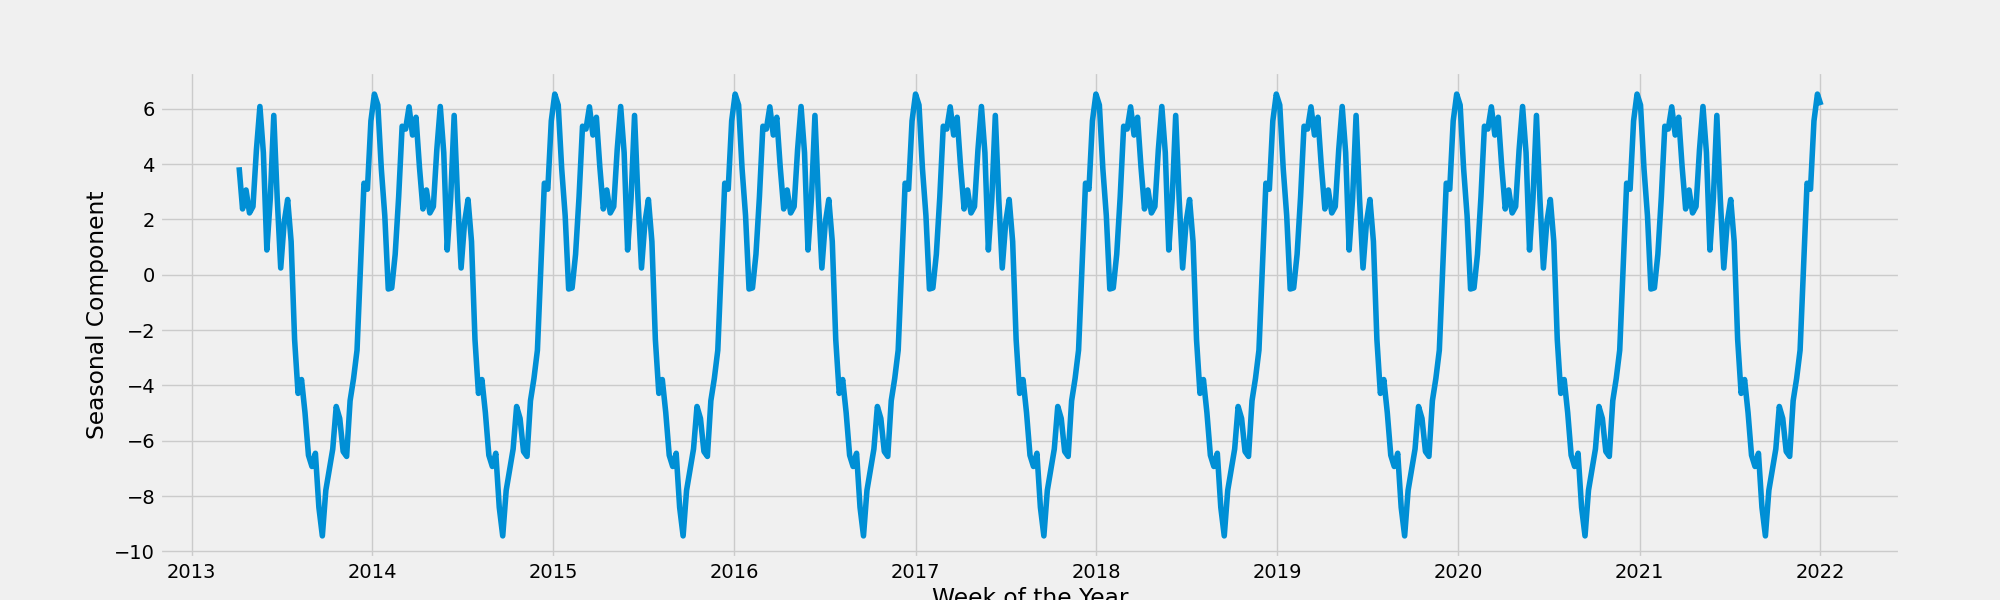
\includegraphics[width=0.8\textwidth]{data/Figures/ARIMA/SeasonalDecompose.png}
    \caption[Seasonal part of the decomposed data]{Seasonal part of the decomposed data}\label{fig:SeasonalDecompose}
\end{figure}

Examining Figure~\ref{fig:SeasonalDecompose} we can see a clear seasonal trend which seems to be repeating itself every 12 months. This could indicate that we should add a seasonal part to the model. As the data is recorded weekly, the $s$ should be 52. \textcite{hyndman_athanasopoulos_2021} mentions that working with weekly data can prove difficult for the ARIMA model to handle as there are, on average, 52.18 weeks in a year, which is not an integer. Nevertheless, we will try to fit a SARIMA model with $s=52$ and compare the AIC and mean squared error of the predictions to the non-seasonal ARIMA model. 

The seasonal part of the ARIMA model also contains $PDQ$ which corresponds to the $pdq$ in the non-seasonal ARIMA model in that they describe the number of seasonal autoregressive terms, the number of seasonal differences, and the number of seasonal moving average terms. In order to determine these terms, we can use the same method as we did for the non-seasonal ARIMA model, namely examine the ACF and PACF plots, but this time for the seasonally differenced data. We can also perform a grid search for the different combinations of AR and MA terms, and in that way obtain the optimal model.

\subsubsection{Exogenous Variables}
One last way to expand on the ARIMA model in order to make it more accurate is to include one or more exogenous variables. This is especially useful if there is some external data that might affect the time series. In our case we suspected that the price of Salmon might be affected by the price of other seafood, as well as the Norwegian Krone. We therefore decided to add these to our dataset and see if it would improve the accuracy of the model.

In order to measure the accuracy of these exogenous variables, we can follow the same procedure as before and compare both the AIC of different models as well as the root mean squared error of the predictions. Comparing the RMSE will probably prove to be a more accurate way of examining the accuracy of the models as AIC cannot handle different levels of differencing and will not work well to compare ARIMA with Tensorflow.~\parencite{brownlee_2017}
\subsection{LSTM --- Tensorflow}\label{Tensorflow_Methodology}
In order to apply the data to a LSTM model, we need to define the different parameters of the model. As a LSTM model consists of an input layer, a hidden layer, and an output layer, we need to define the number of neurons in each layer.

\begin{figure}[H]
    \centering
    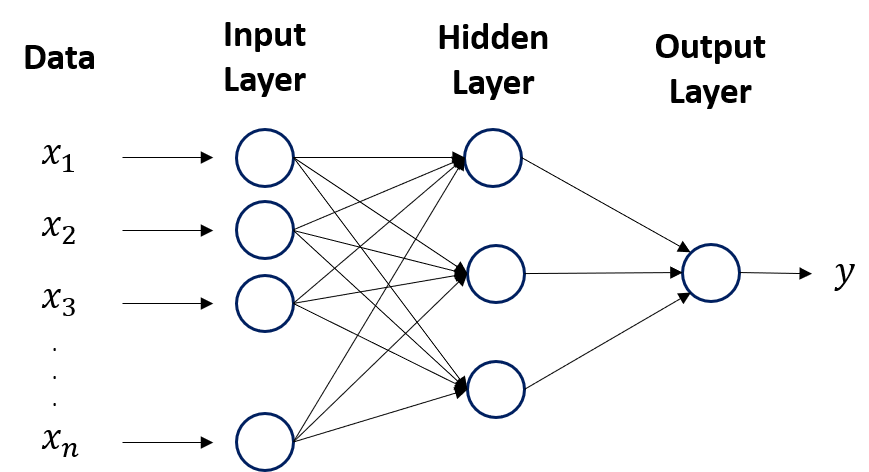
\includegraphics[width=0.8\textwidth]{data/Figures/Neural networks/Layers_lstm.png}
    \caption[Example of the different layers in an LSTM model.]{Example of the different layers in an LSTM model.~\cite{towardsai_2020}}\label{fig:Layers}
\end{figure}
